\chapter{Conclusions}
\label{chap:conclusions}

\setlength{\epigraphwidth}{1.0\textwidth}
\epigraph{No one involved in computers would ever say that a certain amount of memory is enough for all time.}{--- Bill Gates, commenting on the perhaps most famous remark attributed to him}

In this work we examined the applicability of the Lossy Counting algorithm
that was designed to deliver approximate frequency counts over a stream of
input items, to perform on-the-fly filtration of phrase pairs extracted in
the process of phrase table creation in Statistical Machine Translation systems.

To tackle this task, we implemented a software tool that builds a complete phrase
translation table with maximum likelihood scores derived from the frequency
counts as approximated by the lossy counting of phrase pairs extracted from
parallel corpora.
Because internally the Lossy Counting algorithm splits the input stream into
epochs, we dubbed our tool \emph{eppex}, an acronym for \emph{epochal phrase
pairs extractor}.

On top of the standard instantiation of the Lossy Counting algorithm with
\emph{support} and \emph{error} thresholds, we devised a more intuitive interface
to invoke \eppex{}: the \emph{positive} and \emph{negative} limits that
directly relate to the true frequencies of the extracted phrase pairs.
We show the relation of phrase table pruning activated with these limits
to the existing criterion of \emph{count-based pruning}.
We also discussed the impact of various settings of these limits on the memory
demands and output size of the epochal extraction: especially, we stressed
that there is no direct relation between the degree of pruning and the amount
of memory consumed by the program.

We performed a series of the experimental phrase table extractions and carefully
benchmarked the performance of \eppex{} and of a baseline system for phrase
table construction, for which we chose the \emph{phrase-extract} toolkit from
an open-source SMT system, Moses.
Moreover, in our experiments, we also included a popular tool for phrase table
pruning that is shipped with Moses, the significance filter or \emph{sigfilter}
for short.

The results we obtained, showed, that \eppex{} was capable of prune off
substantial amounts of phrase pairs (up to 95\% of the phrase table) without
a significant loss in the ultimate translation quality as confirmed by the
automatic evaluation measure BLEU.
The differences between the baseline and \eppex{} scores were below
0.6~points of BLEU.
In fact, \eppex{} often scored slightly better than the baseline,
although we observed that, when the phrase tables were treated with
state-of-the-art discounting techniques, the baseline performed better.

The \emph{sigfilter} tool seemed to perform slightly better than \eppex{}
in the case of a French-English translation model based on massive training
data with only a single input factor and a language model that was simply
derived from the target side of the parallel corpus.
By contrast, in the case of a two-factored, Czech-English translation model with
the proper language models, slightly better scores were obtained by \eppex{}.

Definitely the biggest advantage of \eppex{}, when compared to the baseline
system, is its runtime performance.
As \Fref{fig:conclusions-cs-en} illustrates, \eppex{} was capable of building
the complete phrase table twice as fast as the most competitive baseline
configuration and with several times less CPU consumption.
On the other hand, \eppex{} requires a considerable amount of RAM to proceed,
while the baseline in its default configuration aims at utilizing as little RAM
as possible.
Therefore, we consider \eppex{} to be a viable alternative to the \emph{phrase-extract}
toolkit rather than a definitive replacement.

\begin{figure}[!htb]
  \centering
  % GNUPLOT: LaTeX picture with Postscript
\begingroup
  \makeatletter
  \providecommand\color[2][]{%
    \GenericError{(gnuplot) \space\space\space\@spaces}{%
      Package color not loaded in conjunction with
      terminal option `colourtext'%
    }{See the gnuplot documentation for explanation.%
    }{Either use 'blacktext' in gnuplot or load the package
      color.sty in LaTeX.}%
    \renewcommand\color[2][]{}%
  }%
  \providecommand\includegraphics[2][]{%
    \GenericError{(gnuplot) \space\space\space\@spaces}{%
      Package graphicx or graphics not loaded%
    }{See the gnuplot documentation for explanation.%
    }{The gnuplot epslatex terminal needs graphicx.sty or graphics.sty.}%
    \renewcommand\includegraphics[2][]{}%
  }%
  \providecommand\rotatebox[2]{#2}%
  \@ifundefined{ifGPcolor}{%
    \newif\ifGPcolor
    \GPcolorfalse
  }{}%
  \@ifundefined{ifGPblacktext}{%
    \newif\ifGPblacktext
    \GPblacktexttrue
  }{}%
  % define a \g@addto@macro without @ in the name:
  \let\gplgaddtomacro\g@addto@macro
  % define empty templates for all commands taking text:
  \gdef\gplbacktext{}%
  \gdef\gplfronttext{}%
  \makeatother
  \ifGPblacktext
    % no textcolor at all
    \def\colorrgb#1{}%
    \def\colorgray#1{}%
  \else
    % gray or color?
    \ifGPcolor
      \def\colorrgb#1{\color[rgb]{#1}}%
      \def\colorgray#1{\color[gray]{#1}}%
      \expandafter\def\csname LTw\endcsname{\color{white}}%
      \expandafter\def\csname LTb\endcsname{\color{black}}%
      \expandafter\def\csname LTa\endcsname{\color{black}}%
      \expandafter\def\csname LT0\endcsname{\color[rgb]{1,0,0}}%
      \expandafter\def\csname LT1\endcsname{\color[rgb]{0,1,0}}%
      \expandafter\def\csname LT2\endcsname{\color[rgb]{0,0,1}}%
      \expandafter\def\csname LT3\endcsname{\color[rgb]{1,0,1}}%
      \expandafter\def\csname LT4\endcsname{\color[rgb]{0,1,1}}%
      \expandafter\def\csname LT5\endcsname{\color[rgb]{1,1,0}}%
      \expandafter\def\csname LT6\endcsname{\color[rgb]{0,0,0}}%
      \expandafter\def\csname LT7\endcsname{\color[rgb]{1,0.3,0}}%
      \expandafter\def\csname LT8\endcsname{\color[rgb]{0.5,0.5,0.5}}%
    \else
      % gray
      \def\colorrgb#1{\color{black}}%
      \def\colorgray#1{\color[gray]{#1}}%
      \expandafter\def\csname LTw\endcsname{\color{white}}%
      \expandafter\def\csname LTb\endcsname{\color{black}}%
      \expandafter\def\csname LTa\endcsname{\color{black}}%
      \expandafter\def\csname LT0\endcsname{\color{black}}%
      \expandafter\def\csname LT1\endcsname{\color{black}}%
      \expandafter\def\csname LT2\endcsname{\color{black}}%
      \expandafter\def\csname LT3\endcsname{\color{black}}%
      \expandafter\def\csname LT4\endcsname{\color{black}}%
      \expandafter\def\csname LT5\endcsname{\color{black}}%
      \expandafter\def\csname LT6\endcsname{\color{black}}%
      \expandafter\def\csname LT7\endcsname{\color{black}}%
      \expandafter\def\csname LT8\endcsname{\color{black}}%
    \fi
  \fi
  \setlength{\unitlength}{0.0500bp}%
  \begin{picture}(7200.00,5040.00)%
    \gplgaddtomacro\gplbacktext{%
      \csname LTb\endcsname%
      \put(814,440){\makebox(0,0)[r]{\strut{} 0}}%
      \put(814,1097){\makebox(0,0)[r]{\strut{} 5}}%
      \put(814,1753){\makebox(0,0)[r]{\strut{} 10}}%
      \put(814,2410){\makebox(0,0)[r]{\strut{} 15}}%
      \put(814,3066){\makebox(0,0)[r]{\strut{} 20}}%
      \put(814,3723){\makebox(0,0)[r]{\strut{} 25}}%
      \put(814,4379){\makebox(0,0)[r]{\strut{} 30}}%
      \put(1941,220){\makebox(0,0){\strut{}def. bas.}}%
      \put(2937,220){\makebox(0,0){\strut{}opt. bas.}}%
      \put(3932,220){\makebox(0,0){\strut{}ep. zero}}%
      \put(4928,220){\makebox(0,0){\strut{}ep. def.}}%
      \put(6055,440){\makebox(0,0)[l]{\strut{} 0}}%
      \put(6055,1228){\makebox(0,0)[l]{\strut{} 10}}%
      \put(6055,2016){\makebox(0,0)[l]{\strut{} 20}}%
      \put(6055,2803){\makebox(0,0)[l]{\strut{} 30}}%
      \put(6055,3591){\makebox(0,0)[l]{\strut{} 40}}%
      \put(6055,4379){\makebox(0,0)[l]{\strut{} 50}}%
      \put(176,2409){\rotatebox{-270}{\makebox(0,0){\strut{}CPU/wallclock time (hours)}}}%
      \put(6692,2409){\rotatebox{-270}{\makebox(0,0){\strut{}virtual memory peak (GB)}}}%
      \put(3434,4709){\makebox(0,0){\strut{}Runtime benchmarking figures (Cs-En dataset)}}%
    }%
    \gplgaddtomacro\gplfronttext{%
      \csname LTb\endcsname%
      \put(2398,4206){\makebox(0,0)[r]{\strut{}clock time}}%
      \csname LTb\endcsname%
      \put(2398,3986){\makebox(0,0)[r]{\strut{}cpu time}}%
      \csname LTb\endcsname%
      \put(4573,4206){\makebox(0,0)[r]{\strut{}vm peak}}%
    }%
    \gplbacktext
    \put(0,0){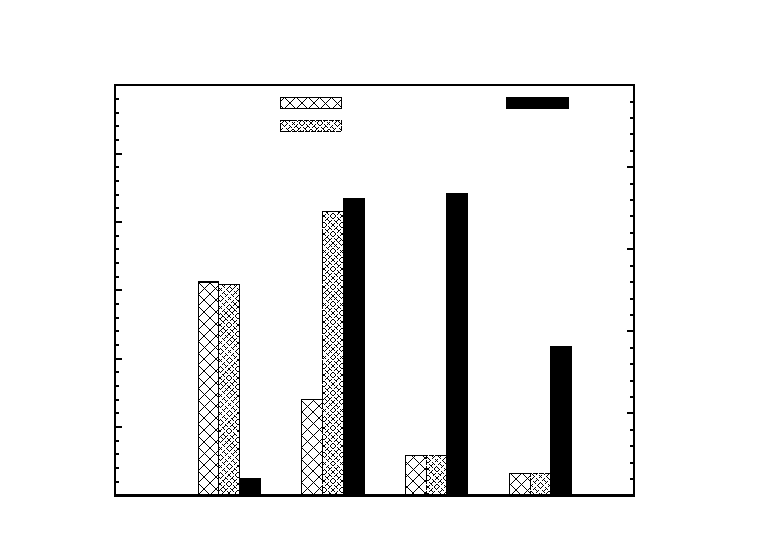
\includegraphics{conclusions-cs-en}}%
    \gplfronttext
  \end{picture}%
\endgroup

  \caption{
    Summary of the runtime benchmarking figures for the most relevant experiments
    with the Czech-English dataset (from left to right): baseline with the default
    parameters, baseline using multiple cores and large memory buffer, \eppex{}
    with no pruning and the \eppex{} with pruning configuration that achieved the best
    BLEU score of all experiments (labeled \emph{eppex defensive}).
  }
  \label{fig:conclusions-cs-en}
\end{figure}

\section{Future work}

We are aware, that in its current state, \eppex{} is a usable tool,
but a potential user of \eppex{} could be discouraged by the lack of some
finer control over its memory demands incurred during
runtime.

%\footnote{Without neglecting the importance of good program design,
%we cannot disregard the empirically determined principle that often the easiest
%and also cheapest solution to the performance limitations imposed by hardware
%is to buy better hardware. After all, no certain amount of memory is enough
%for all time.}

Addressing this possible concern, we see two possible ways to improve \eppex{}:
\begin{enumerate}
  \item Provide the user with a method to properly determine the maximum amount
    of memory that \eppex{} would require to process a particular training data.
  \item Provide the user with an option to set a limit on the maximum amount
    of memory utilized by the program.
\end{enumerate}

% VM peak estimation
In \Sref{sec:eppex-memory-demands} we already sketched a possible approach of how to determine
the memory peak of epochal extraction with a given pruning configuration and given input data.
However, it is hard to know whether this approach could be enhanced to offer
a more precise estimation than the 20\% overestimate based on the 25\% of training
data that we achieved in our initial experiments, and how consistent this estimation
could be made.

% Iterative deepening.
Point two has two possible approaches.
The first approach is to make the program aware of its memory consumption and implement
some means of resolving the situation when all available memory is exhausted.
The second approach is to control program memory consumption from outside:
as soon as its memory consumption exceeds a predefined limit, it can simply be terminated, 
and run again with harsher pruning (e.g. by raising the positive limit).
Obviously, the second approach does not require any changes to the existing version of
program, just a bit of scripting.

% Incremental training.
Besides finer control over memory consumption, yet another problem that could
be addressed in future work on \eppex{}, is the support for \emph{incremental
training}.
With new parallel data becoming available every year, more and more researchers seek
the means to retrain their translation models without running the whole
training process from scratch.

In a way, \eppex{} already helps work around this problem: by making the training
process much faster, the need to avoid rerunning the training process is somewhat
lowered.
However, a more straight-forward solution should be also possible.
Given that phrase tables usually contain the frequency counts of phrase pairs,
these frequencies could be used to initialize the internal Lossy Counting data
memory and the epochal extraction could then proceed by processing only the new
training data.
